\documentclass[12pt,a4paper]{scrartcl}\usepackage[]{graphicx}\usepackage[]{color}
% maxwidth is the original width if it is less than linewidth
% otherwise use linewidth (to make sure the graphics do not exceed the margin)
\makeatletter
\def\maxwidth{ %
  \ifdim\Gin@nat@width>\linewidth
    \linewidth
  \else
    \Gin@nat@width
  \fi
}
\makeatother

\definecolor{fgcolor}{rgb}{0.345, 0.345, 0.345}
\newcommand{\hlnum}[1]{\textcolor[rgb]{0.686,0.059,0.569}{#1}}%
\newcommand{\hlstr}[1]{\textcolor[rgb]{0.192,0.494,0.8}{#1}}%
\newcommand{\hlcom}[1]{\textcolor[rgb]{0.678,0.584,0.686}{\textit{#1}}}%
\newcommand{\hlopt}[1]{\textcolor[rgb]{0,0,0}{#1}}%
\newcommand{\hlstd}[1]{\textcolor[rgb]{0.345,0.345,0.345}{#1}}%
\newcommand{\hlkwa}[1]{\textcolor[rgb]{0.161,0.373,0.58}{\textbf{#1}}}%
\newcommand{\hlkwb}[1]{\textcolor[rgb]{0.69,0.353,0.396}{#1}}%
\newcommand{\hlkwc}[1]{\textcolor[rgb]{0.333,0.667,0.333}{#1}}%
\newcommand{\hlkwd}[1]{\textcolor[rgb]{0.737,0.353,0.396}{\textbf{#1}}}%
\let\hlipl\hlkwb

\usepackage{framed}
\makeatletter
\newenvironment{kframe}{%
 \def\at@end@of@kframe{}%
 \ifinner\ifhmode%
  \def\at@end@of@kframe{\end{minipage}}%
  \begin{minipage}{\columnwidth}%
 \fi\fi%
 \def\FrameCommand##1{\hskip\@totalleftmargin \hskip-\fboxsep
 \colorbox{shadecolor}{##1}\hskip-\fboxsep
     % There is no \\@totalrightmargin, so:
     \hskip-\linewidth \hskip-\@totalleftmargin \hskip\columnwidth}%
 \MakeFramed {\advance\hsize-\width
   \@totalleftmargin\z@ \linewidth\hsize
   \@setminipage}}%
 {\par\unskip\endMakeFramed%
 \at@end@of@kframe}
\makeatother

\definecolor{shadecolor}{rgb}{.97, .97, .97}
\definecolor{messagecolor}{rgb}{0, 0, 0}
\definecolor{warningcolor}{rgb}{1, 0, 1}
\definecolor{errorcolor}{rgb}{1, 0, 0}
\newenvironment{knitrout}{}{} % an empty environment to be redefined in TeX

\usepackage{alltt}
\usepackage[utf8]{inputenc}
\usepackage{amsmath}
\usepackage{graphicx}
\usepackage{tikz}
%\usepackage{silence}
\usepackage{mdframed}
%\WarningFilter{mdframed}{You got a bad break}
\usepackage[colorinlistoftodos]{todonotes}
\usepackage{listings}
\usepackage{color}
\colorlet{exampcol}{blue!10}
\usepackage{multicol}
\usepackage{booktabs}


\usepackage{tcolorbox}


\usepackage{setspace}
%\doublespacing

\usepackage[noanswer]{exercise}%[noanswer]
\renewcommand{\ExerciseHeaderTitle}{\quad---\quad \color{orange!70!black}\ExerciseTitle}


\usepackage[autostyle, english = american]{csquotes}
\MakeOuterQuote{"}

\usepackage{hyperref}
\hypersetup{
    colorlinks,
    citecolor=black,
    filecolor=black,
    linkcolor=blue,
    urlcolor=blue
}

\title{R-StatProgamming with functions in R}
\date{\today}
\author{Timoth\'ee Bonnet, BDSI}
\IfFileExists{upquote.sty}{\usepackage{upquote}}{}
\begin{document}



\maketitle

On Friday 03/04/2020 I will be presenting this tutorial live on Zoom. (ask by email/Slack if you do not know how to use Zoom.)

If you have any trouble going through this tutorial then or at a different time you can chat about it on Slack ( rsb-r-stats-biology.slack.com , if you are not a member but would like to be, drop me an email) or email me at \href{mailto:timotheebonnetc@gmail.com}{timotheebonnetc@gmail.com}.

If you do not attend the Zoom meeting but would like to receive credit through the \href{https://wattlecourses.anu.edu.au/enrol/index.php?id=23938}{COS Career Development Framework} program I need you to complete three exercises of your choice. Send me your answers via Slack or email. It does not have to be correct on the first try and you are welcome to get in touch if you are completely stuck. I will provide feedback to help you complete exercises you want to do.

In this tutorial you will learn:

\begin{itemize}
    \item How unexplained variation in a response variable can compromise statistical inference when that variation is structured.
    \item How fixed and random effects can correct for structured variation in the response variable.
    \item How to fit mixed-effects models in R.
    \item How to choose between fixed and random effects.
    \item Extract and interpret mixed models output.
    \item Test for the statistical significance of a random effect.
\end{itemize}

\tableofcontents
\ListOfExerciseInToc
\ExerciseLevelInToc{subsubsection}

\clearpage

\section{The dangers of unexplained variation}
Imagine you have measured how much a plant species is attacked by big herbivores as a function of how many thorns the plant grows on stems. You have collected data in 5 locations and visualise the relationship between herbivory and quantity of thorns (in arbitrary units):
\begin{center}
  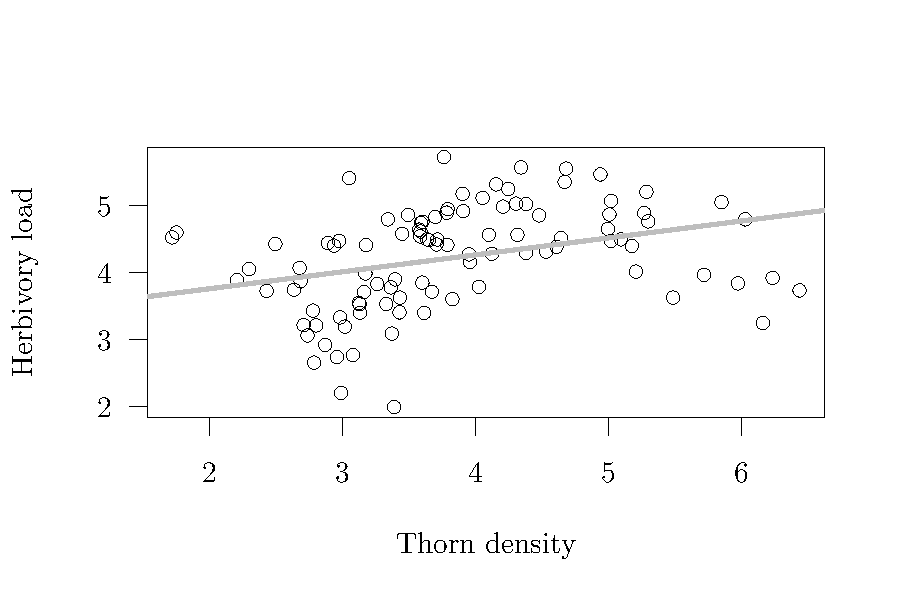
\includegraphics[width=0.8\textwidth]{figures/graph0-1.pdf}
\end{center}

It looks like the more a plant has thorns, the more it is eaten. Let's check that by fitting a linear regression.

\begin{knitrout}
\definecolor{shadecolor}{rgb}{0.969, 0.969, 0.969}\color{fgcolor}\begin{kframe}
\begin{alltt}
\hlstd{thorns} \hlkwb{<-} \hlkwd{read.csv}\hlstd{(}\hlkwc{file} \hlstd{=} \hlstr{"Data/thorndata.csv"}\hlstd{,} \hlkwc{header}\hlstd{=}\hlnum{TRUE}\hlstd{)}
\hlkwd{str}\hlstd{(thorns)}
\end{alltt}
\begin{verbatim}
## 'data.frame':	100 obs. of  3 variables:
##  $ herbivory   : num  4.53 4.6 3.89 4.05 3.73 ...
##  $ thorndensity: num  1.72 1.75 2.2 2.3 2.43 ...
##  $ site        : Factor w/ 5 levels "a","b","c","d",..: 1 1 1 1 1 1 1 1 1 1 ...
\end{verbatim}
\begin{alltt}
\hlstd{model_0} \hlkwb{<-} \hlkwd{lm}\hlstd{(herbivory} \hlopt{~} \hlstd{thorndensity,} \hlkwc{data} \hlstd{= thorns)}
\hlkwd{summary}\hlstd{(model_0)}
\end{alltt}
\begin{verbatim}
## 
## Call:
## lm(formula = herbivory ~ thorndensity, data = thorns)
## 
## Residuals:
##     Min      1Q  Median      3Q     Max 
## -2.1162 -0.5183  0.0821  0.5435  1.5193 
## 
## Coefficients:
##              Estimate Std. Error t value Pr(>|t|)    
## (Intercept)    3.2564     0.2854   11.41  < 2e-16 ***
## thorndensity   0.2524     0.0717    3.52  0.00066 ***
## ---
## Signif. codes:  0 '***' 0.001 '**' 0.01 '*' 0.05 '.' 0.1 ' ' 1
## 
## Residual standard error: 0.725 on 98 degrees of freedom
## Multiple R-squared:  0.112,	Adjusted R-squared:  0.103 
## F-statistic: 12.4 on 1 and 98 DF,  p-value: 0.000657
\end{verbatim}
\end{kframe}
\end{knitrout}
This model confirms a positive relationship between how much a plant has thorns and how much it is consumed by herbivores; which is counter-intuitive.

The twist is that data were collected in 5 different sites, that our two variables have different mean values in different sites, and that our model is not aware of that. 
We can see the structure in the data by coloring the points by site:
\begin{center}
  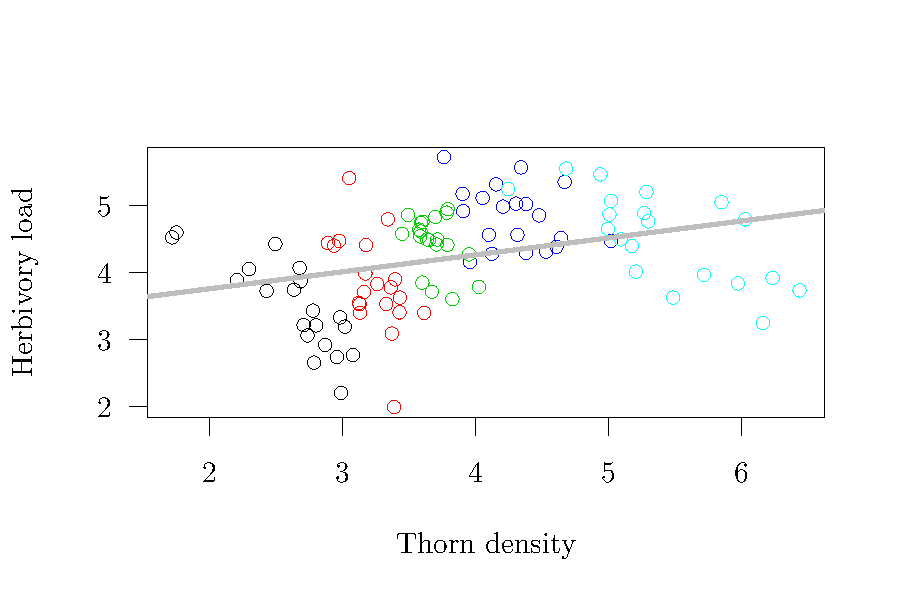
\includegraphics[width=0.8\textwidth]{figures/graph1-1.pdf}
\end{center}

Maybe you remember that in a linear model (such as a linear regression) we assume that the residuals follow a normal distribution without any structure (homoscedasticity, independence\dots).
It is not easy to see patterns by just ploting the residuals:
\begin{knitrout}
\definecolor{shadecolor}{rgb}{0.969, 0.969, 0.969}\color{fgcolor}\begin{kframe}
\begin{alltt}
\hlkwd{plot}\hlstd{(}\hlkwd{residuals}\hlstd{(model_0))}
\end{alltt}
\end{kframe}
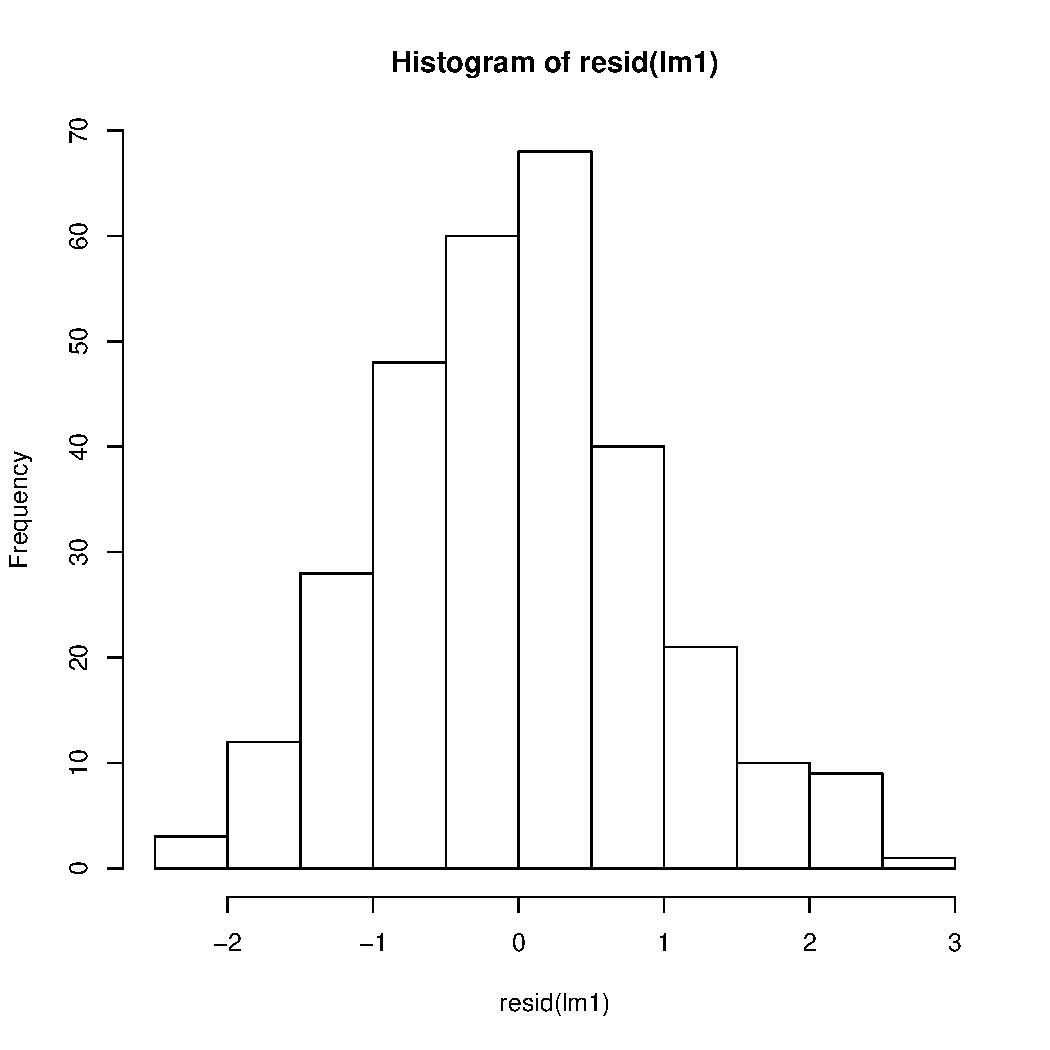
\includegraphics[width=\maxwidth]{figure/unnamed-chunk-3-1} 

\end{knitrout}

However, in our case, we have data about the missing variable that structure residuals, so we can see clearly that residuals are distributed with structure:
\begin{knitrout}
\definecolor{shadecolor}{rgb}{0.969, 0.969, 0.969}\color{fgcolor}\begin{kframe}
\begin{alltt}
\hlkwd{plot}\hlstd{(thorns}\hlopt{$}\hlstd{site,} \hlkwd{residuals}\hlstd{(model_0))}
\end{alltt}
\end{kframe}
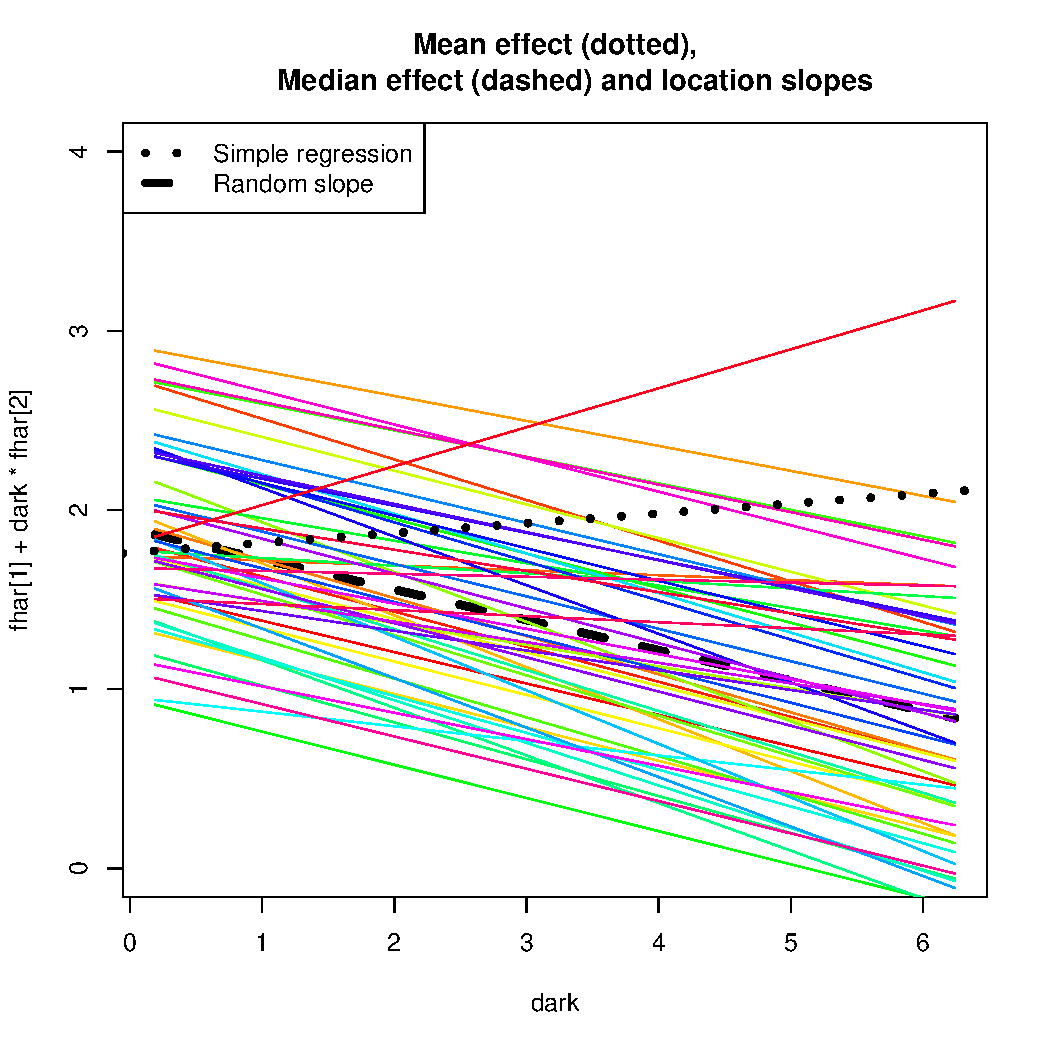
\includegraphics[width=\maxwidth]{figure/unnamed-chunk-4-1} 

\end{knitrout}

We can correct the problem by fititng site in the mode:
\begin{knitrout}
\definecolor{shadecolor}{rgb}{0.969, 0.969, 0.969}\color{fgcolor}\begin{kframe}
\begin{alltt}
\hlstd{model_1} \hlkwb{<-} \hlkwd{lm}\hlstd{(herbivory} \hlopt{~} \hlstd{thorndensity} \hlopt{+} \hlstd{site,} \hlkwc{data} \hlstd{= thorns)}
\hlkwd{summary}\hlstd{(model_1)}
\end{alltt}
\begin{verbatim}
## 
## Call:
## lm(formula = herbivory ~ thorndensity + site, data = thorns)
## 
## Residuals:
##     Min      1Q  Median      3Q     Max 
## -1.6877 -0.2889  0.0498  0.2492  1.3968 
## 
## Coefficients:
##              Estimate Std. Error t value Pr(>|t|)    
## (Intercept)     6.047      0.387   15.62  < 2e-16 ***
## thorndensity   -0.975      0.141   -6.90  6.0e-10 ***
## siteb           0.940      0.176    5.33  6.6e-07 ***
## sitec           1.996      0.215    9.30  5.8e-15 ***
## sited           2.971      0.281   10.56  < 2e-16 ***
## sitee           3.767      0.422    8.93  3.5e-14 ***
## ---
## Signif. codes:  0 '***' 0.001 '**' 0.01 '*' 0.05 '.' 0.1 ' ' 1
## 
## Residual standard error: 0.488 on 94 degrees of freedom
## Multiple R-squared:  0.615,	Adjusted R-squared:  0.595 
## F-statistic:   30 on 5 and 94 DF,  p-value: <2e-16
\end{verbatim}
\end{kframe}
\end{knitrout}

Now we see a negative relationship between thorn density and herbivory. 

That model corresponds to the plot below:
\begin{center}
  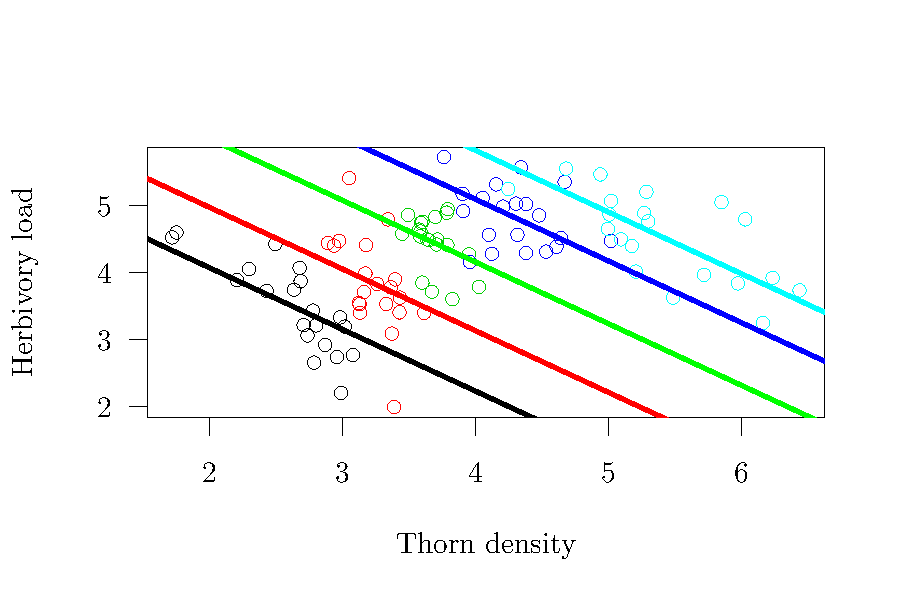
\includegraphics[width=0.8\textwidth]{figures/graph2-1.pdf}
\end{center}
We have 5 parallel regression lines, one for each site. Differences in the mean values within each sites are accounted for but we estimate the common slope across all sites.

The residuals of that model are more clearly without pattern:
\begin{knitrout}
\definecolor{shadecolor}{rgb}{0.969, 0.969, 0.969}\color{fgcolor}\begin{kframe}
\begin{alltt}
\hlkwd{plot}\hlstd{(}\hlkwd{residuals}\hlstd{(model_1))}
\end{alltt}
\end{kframe}
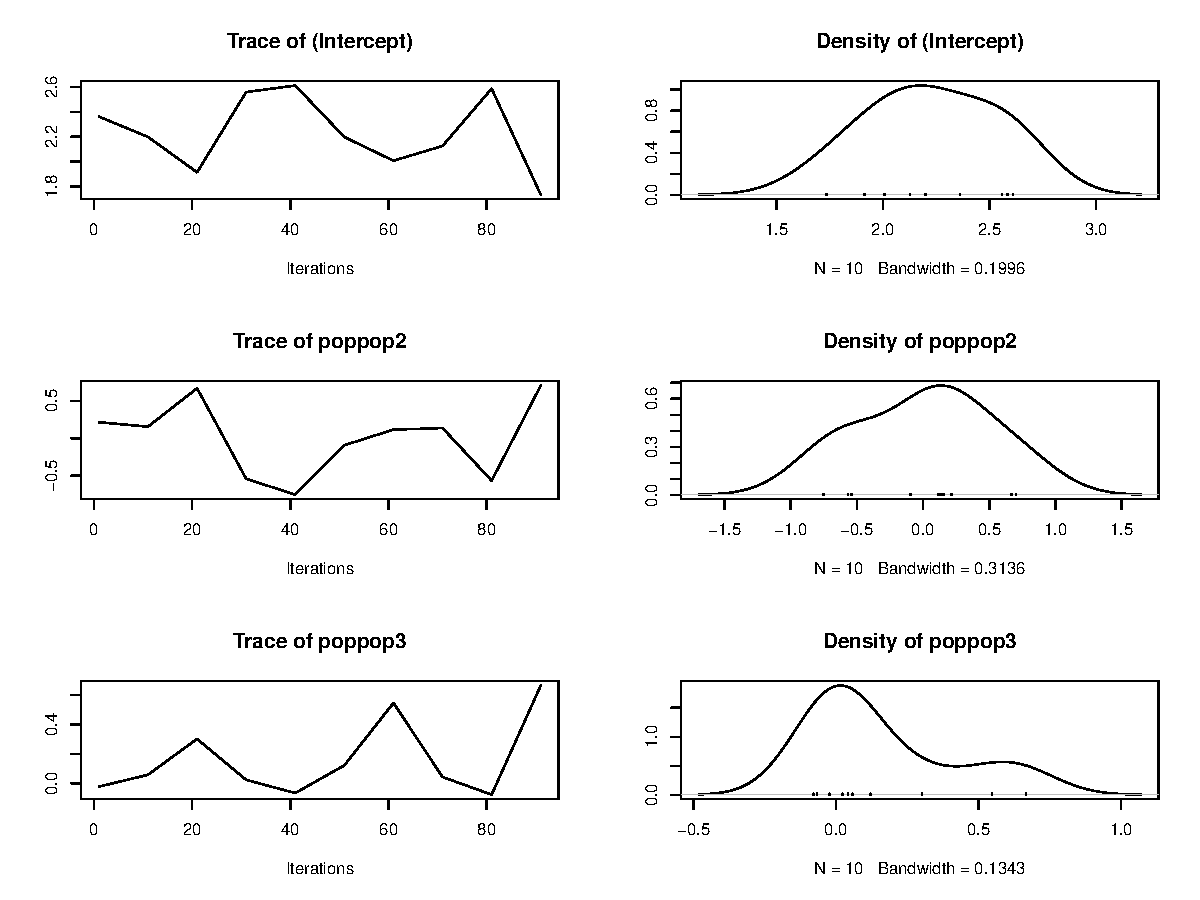
\includegraphics[width=\maxwidth]{figure/unnamed-chunk-6-1} 
\begin{kframe}\begin{alltt}
\hlkwd{plot}\hlstd{(thorns}\hlopt{$}\hlstd{site,} \hlkwd{residuals}\hlstd{(model_1))}
\end{alltt}
\end{kframe}
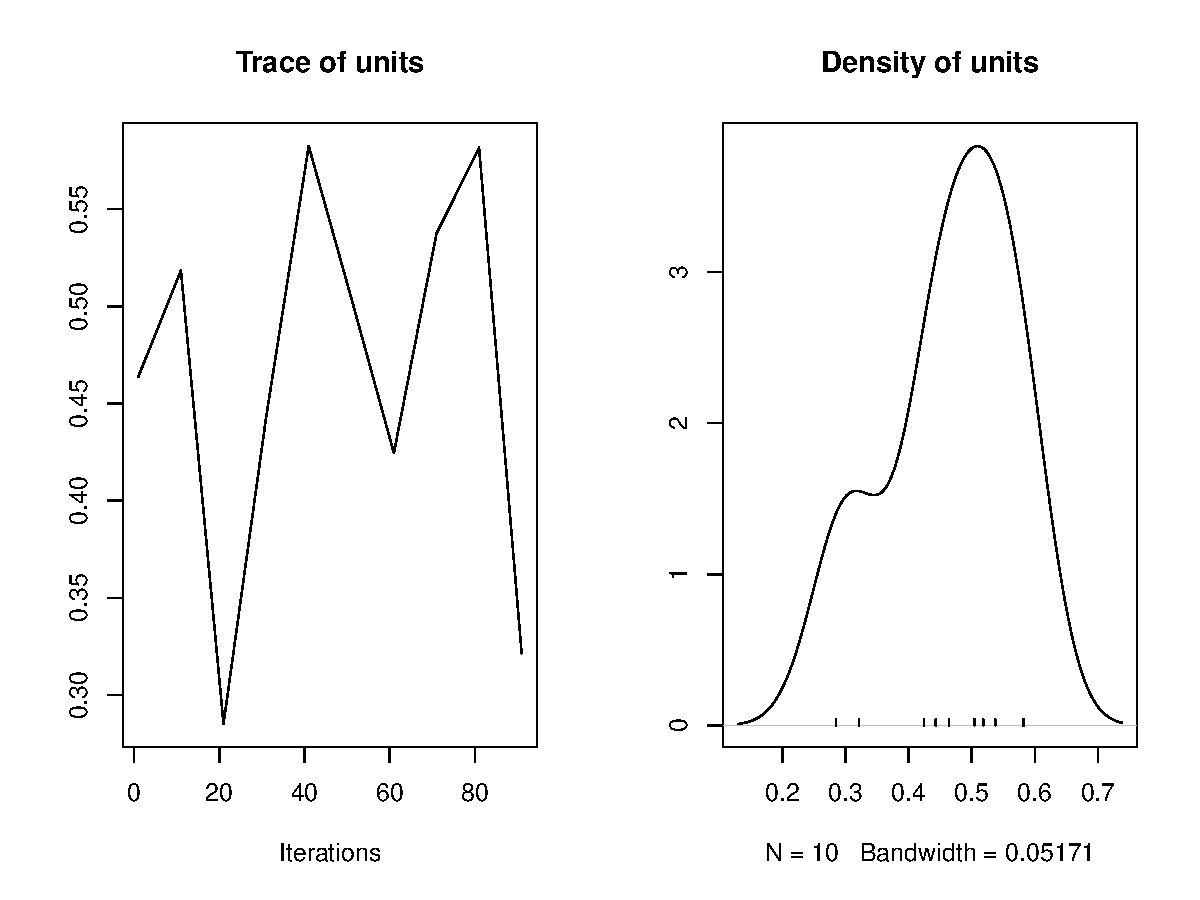
\includegraphics[width=\maxwidth]{figure/unnamed-chunk-6-2} 

\end{knitrout}


Note that in the summary of model\_1 we have 4 parameter estimates we did not really care about: the deviations of four site relative to the fifth site. It does not hurt to have them there, but we are not really interested in them because 1) we did not have questions about how sites vary in herbivory, 2) site is just a grouping factor and differences between sites are probably due to numerous processes we have not measured. Given our ignorance on what makes sites different, the values of site effects are essentially random; we fit site only to get a correct inference but do not learn much from the estimated effects of sites.

\section{Fitting random effects}

Now imagine a larger research setting where you would have collected data in 50 sites for a response variable and a predictor.


Check what happens if we approach the problem as in the thorn example:
\begin{knitrout}
\definecolor{shadecolor}{rgb}{0.969, 0.969, 0.969}\color{fgcolor}\begin{kframe}
\begin{alltt}
\hlstd{biggerdata} \hlkwb{<-} \hlkwd{read.csv}\hlstd{(}\hlstr{"Data/biggerdata.csv"}\hlstd{)}
\hlkwd{str}\hlstd{(biggerdata)}
\end{alltt}
\begin{verbatim}
## 'data.frame':	10000 obs. of  3 variables:
##  $ predictor: num  1.72 1.88 2.78 2.04 2.06 ...
##  $ response : num  3.252 1.476 0.143 2.248 0.489 ...
##  $ site     : Factor w/ 50 levels "s1","s10","s11",..: 25 3 17 46 47 14 4 47 10 27 ...
\end{verbatim}
\begin{alltt}
\hlstd{bdmodel} \hlkwb{<-} \hlkwd{lm}\hlstd{(response} \hlopt{~} \hlstd{predictor} \hlopt{+} \hlstd{site,} \hlkwc{data} \hlstd{= biggerdata)}
\end{alltt}
\end{kframe}
\end{knitrout}
\begin{knitrout}
\definecolor{shadecolor}{rgb}{0.969, 0.969, 0.969}\color{fgcolor}\begin{kframe}
\begin{alltt}
\hlkwd{summary}\hlstd{(bdmodel)}
\end{alltt}
\end{kframe}
\end{knitrout}

You will find it is a bit of a mess. We have 49 parameter estimates for sites, but we do not really care about those effects, they are essentially random to us. It would be more efficient to fit site as a random effect!

To do so, load (and install if needed) the package \texttt{lme4}. 
\begin{knitrout}
\definecolor{shadecolor}{rgb}{0.969, 0.969, 0.969}\color{fgcolor}\begin{kframe}
\begin{alltt}
\hlkwd{library}\hlstd{(lme4)}
\end{alltt}


{\ttfamily\noindent\itshape\color{messagecolor}{\#\# Loading required package: Matrix}}\end{kframe}
\end{knitrout}
Then you can copy paste the model we called bdmodel, and change two things: 1) change \texttt{lm} to \texttt{lmer}; 2) change \texttt{site} to \texttt{(1|site)}:

\begin{knitrout}
\definecolor{shadecolor}{rgb}{0.969, 0.969, 0.969}\color{fgcolor}\begin{kframe}
\begin{alltt}
\hlstd{bdmmixedmodel} \hlkwb{<-} \hlkwd{lmer}\hlstd{(response} \hlopt{~} \hlstd{predictor} \hlopt{+} \hlstd{(}\hlnum{1}\hlopt{|}\hlstd{site),} \hlkwc{data} \hlstd{= biggerdata)}
\end{alltt}
\end{kframe}
\end{knitrout}
That's it, you have fitted a mixed effect model: that is, a model with both fixed and random effect. The syntax (1|something) means that the variable "something" is fitted as a random effect, while the variable "predictor" remains a fixed effect. Check the summary of that model:
\begin{knitrout}
\definecolor{shadecolor}{rgb}{0.969, 0.969, 0.969}\color{fgcolor}\begin{kframe}
\begin{alltt}
\hlkwd{summary}\hlstd{(bdmmixedmodel)}
\end{alltt}
\begin{verbatim}
## Linear mixed model fit by REML ['lmerMod']
## Formula: response ~ predictor + (1 | site)
##    Data: biggerdata
## 
## REML criterion at convergence: 14852
## 
## Scaled residuals: 
##    Min     1Q Median     3Q    Max 
## -3.712 -0.679 -0.011  0.667  3.854 
## 
## Random effects:
##  Groups   Name        Variance Std.Dev.
##  site     (Intercept) 5.930    2.435   
##  Residual             0.248    0.498   
## Number of obs: 10000, groups:  site, 50
## 
## Fixed effects:
##             Estimate Std. Error t value
## (Intercept)  1.96051    0.34499    5.68
## predictor    0.17579    0.00999   17.60
## 
## Correlation of Fixed Effects:
##           (Intr)
## predictor -0.058
\end{verbatim}
\end{kframe}
\end{knitrout}

Now we see a single fixed effect (apart from the intercetp), that of the variable "predictor". The 49 site effects are not there anymore. Where did they go? In the Random effects section, labeled as "site (Intercept)", and instead of seeing 49 effects, we have 50 effects summarized in a single number, namely the variance in those effects: 5.9297. There is a second number, Std.Dev. which in this case is  2.4351, but that is just the standard deviation, that is, the square-root of the variance.

So Variance and Std.Dev. carry exactly the same information: the amount of difference among sites.
Below site, there is a row for Residual, again giving both a Variance and a Std.Dev. This quantifies the variance left unexplained within each site, after removing the variance explained by fixed effects and random effects.


Time for some practice on your own:

\begin{Exercise}[difficulty=1, title={A mixed model for the thorn data set}]
\begin{enumerate}
  \item Load the dataset "thorndata.csv" to fit a linear model of "herbivory" as a function of "thorndensity". What is the estimate for the slope?\\
  \item Add a random effect for site. How does the estimate for the slope changes?\\
  \item How much variation is explained by differences among sites? How much variation remains unexplained within sites?
\end{enumerate}
\end{Exercise}

\begin{Answer}
Part 1.
\begin{knitrout}
\definecolor{shadecolor}{rgb}{0.969, 0.969, 0.969}\color{fgcolor}\begin{kframe}
\begin{alltt}
\hlstd{thorns} \hlkwb{<-} \hlkwd{read.csv}\hlstd{(}\hlstr{"Data/thorndata.csv"}\hlstd{)}
\hlkwd{lm}\hlstd{(herbivory} \hlopt{~} \hlstd{thorndensity,} \hlkwc{data}\hlstd{=thorns)}
\end{alltt}
\begin{verbatim}
## 
## Call:
## lm(formula = herbivory ~ thorndensity, data = thorns)
## 
## Coefficients:
##  (Intercept)  thorndensity  
##        3.256         0.252
\end{verbatim}
\end{kframe}
\end{knitrout}
The slope is 0.2524.\\

Part 2.
\begin{knitrout}
\definecolor{shadecolor}{rgb}{0.969, 0.969, 0.969}\color{fgcolor}\begin{kframe}
\begin{alltt}
\hlkwd{library}\hlstd{(lme4)}
\hlkwd{summary}\hlstd{(}\hlkwd{lmer}\hlstd{(herbivory} \hlopt{~} \hlstd{thorndensity} \hlopt{+} \hlstd{(}\hlnum{1}\hlopt{|}\hlstd{site),} \hlkwc{data}\hlstd{=thorns))}
\end{alltt}
\begin{verbatim}
## Linear mixed model fit by REML ['lmerMod']
## Formula: herbivory ~ thorndensity + (1 | site)
##    Data: thorns
## 
## REML criterion at convergence: 165.3
## 
## Scaled residuals: 
##    Min     1Q Median     3Q    Max 
## -3.488 -0.606  0.109  0.523  2.873 
## 
## Random effects:
##  Groups   Name        Variance Std.Dev.
##  site     (Intercept) 2.129    1.459   
##  Residual             0.238    0.488   
## Number of obs: 100, groups:  site, 5
## 
## Fixed effects:
##              Estimate Std. Error t value
## (Intercept)     7.765      0.844    9.20
## thorndensity   -0.919      0.139   -6.63
## 
## Correlation of Fixed Effects:
##             (Intr)
## thorndensty -0.632
\end{verbatim}
\end{kframe}
\end{knitrout}
The slope is now NULL.\\

Part 3.
\begin{knitrout}
\definecolor{shadecolor}{rgb}{0.969, 0.969, 0.969}\color{fgcolor}\begin{kframe}
\begin{alltt}
\hlkwd{summary}\hlstd{(}\hlkwd{lmer}\hlstd{(herbivory} \hlopt{~} \hlstd{thorndensity} \hlopt{+} \hlstd{(}\hlnum{1}\hlopt{|}\hlstd{site),} \hlkwc{data}\hlstd{=thorns))}
\hlkwd{as.numeric}\hlstd{(}\hlkwd{VarCorr}\hlstd{(}\hlkwd{lmer}\hlstd{(herbivory} \hlopt{~} \hlstd{thorndensity} \hlopt{+} \hlstd{(}\hlnum{1}\hlopt{|}\hlstd{site),} \hlkwc{data}\hlstd{=thorns))}\hlopt{$}\hlstd{site)}
\end{alltt}
\end{kframe}
\end{knitrout}
The variance explained by block is  (careful, if you extract the standard deviation (Std.Dev.) you need to square it to obtain a variance.). There is no measure of uncertainty for the estimate of variance in block. In the \texttt{summmary} the \texttt{Std.Dev.} is simply the square root of \texttt{Variance}.
\end{Answer}


Remember how we went from 49 fixed effect parameters to 1 random effect parameter in the previous example? Doesn't it sound a bit weird? How can we summarize 49 (or 50) numbers in 1. Well, by making one assumption: that these 50 numbers follow a normal distribution, which we define such that its mean is zero. A normal distribution is defined by 2 parameters, the mean and the variance, we fix the mean to zero, so we can describe the distribution with the variance only. 
Let's visualize that distribution:
The model was:
\begin{knitrout}
\definecolor{shadecolor}{rgb}{0.969, 0.969, 0.969}\color{fgcolor}\begin{kframe}
\begin{alltt}
\hlstd{mm0} \hlkwb{<-} \hlkwd{lmer}\hlstd{(response} \hlopt{~} \hlstd{predictor} \hlopt{+} \hlstd{(}\hlnum{1}\hlopt{|}\hlstd{site),} \hlkwc{data}\hlstd{=biggerdata)}
\end{alltt}
\end{kframe}
\end{knitrout}

We can extract the random variance for site as:
\begin{knitrout}
\definecolor{shadecolor}{rgb}{0.969, 0.969, 0.969}\color{fgcolor}\begin{kframe}
\begin{alltt}
\hlstd{rvar} \hlkwb{<-} \hlkwd{as.numeric}\hlstd{(}\hlkwd{VarCorr}\hlstd{(mm0)}\hlopt{$}\hlstd{site)}
\end{alltt}
\end{kframe}
\end{knitrout}

Knowing that most of a normal distribution is contained within +/- 4 times its standard deviation, we can visualize the density distribution of the random effect:
\begin{knitrout}
\definecolor{shadecolor}{rgb}{0.969, 0.969, 0.969}\color{fgcolor}\begin{kframe}
\begin{alltt}
\hlstd{x} \hlkwb{<-} \hlkwd{seq}\hlstd{(}\hlopt{-}\hlnum{4}\hlopt{*}\hlkwd{sqrt}\hlstd{(rvar),}\hlnum{4}\hlopt{*}\hlkwd{sqrt}\hlstd{(rvar),}\hlkwd{sqrt}\hlstd{(rvar)}\hlopt{/}\hlnum{100}\hlstd{)}
\hlkwd{plot}\hlstd{(}\hlkwc{x}\hlstd{=x,} \hlkwc{y}\hlstd{=}\hlkwd{dnorm}\hlstd{(}\hlkwc{x} \hlstd{= x,} \hlkwc{mean} \hlstd{=}\hlnum{0} \hlstd{,} \hlkwc{sd} \hlstd{=} \hlkwd{sqrt}\hlstd{(rvar)),} \hlkwc{type}\hlstd{=}\hlstr{"l"}\hlstd{,}
     \hlkwc{xlab}\hlstd{=} \hlstr{"value of random deviation"}\hlstd{,} \hlkwc{ylab}\hlstd{=}\hlstr{"probability density"}\hlstd{,} \hlkwc{lwd}\hlstd{=}\hlnum{5}\hlstd{)}
\end{alltt}
\end{kframe}
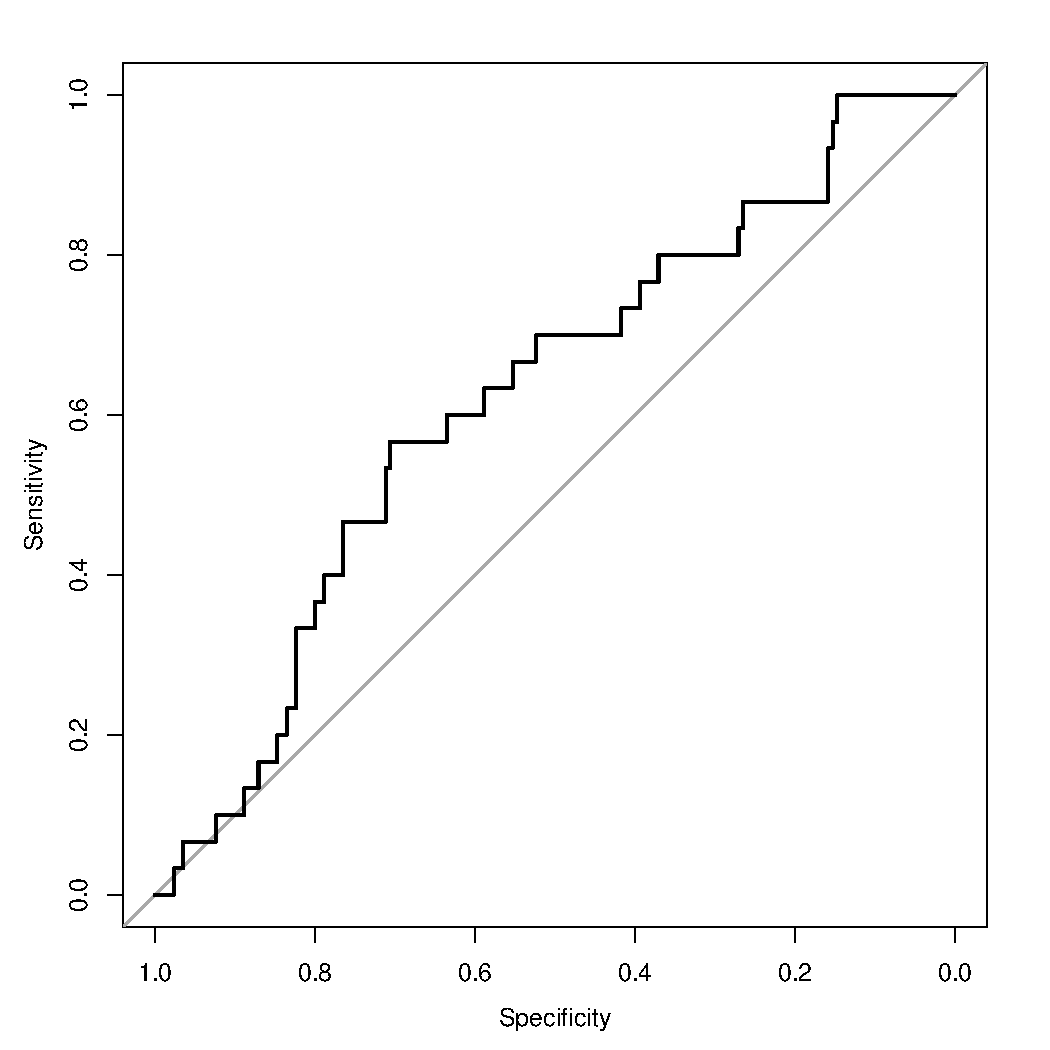
\includegraphics[width=\maxwidth]{figure/unnamed-chunk-18-1} 

\end{knitrout}

The actual random deviation for each site are "kind of" estimated and can be extracted with the function \texttt{ranef()}. In our case \texttt{ranef()} will return 50 values. Let's map them onto the previous plot:

\begin{knitrout}
\definecolor{shadecolor}{rgb}{0.969, 0.969, 0.969}\color{fgcolor}\begin{kframe}
\begin{alltt}
\hlstd{x} \hlkwb{<-} \hlkwd{seq}\hlstd{(}\hlopt{-}\hlnum{4}\hlopt{*}\hlkwd{sqrt}\hlstd{(rvar),}\hlnum{4}\hlopt{*}\hlkwd{sqrt}\hlstd{(rvar),}\hlkwd{sqrt}\hlstd{(rvar)}\hlopt{/}\hlnum{100}\hlstd{)}
\hlkwd{plot}\hlstd{(}\hlkwc{x}\hlstd{=x,} \hlkwc{y}\hlstd{=}\hlkwd{dnorm}\hlstd{(}\hlkwc{x} \hlstd{= x,} \hlkwc{mean} \hlstd{=}\hlnum{0} \hlstd{,} \hlkwc{sd} \hlstd{=} \hlkwd{sqrt}\hlstd{(rvar)),} \hlkwc{type}\hlstd{=}\hlstr{"l"}\hlstd{,}
     \hlkwc{xlab}\hlstd{=} \hlstr{"value of random deviation"}\hlstd{,} \hlkwc{ylab}\hlstd{=}\hlstr{"probability density"}\hlstd{,} \hlkwc{lwd}\hlstd{=}\hlnum{5}\hlstd{)}
\hlkwd{abline}\hlstd{(}\hlkwc{v}\hlstd{=}\hlkwd{unlist}\hlstd{(}\hlkwd{ranef}\hlstd{(mm0)),} \hlkwc{col}\hlstd{=} \hlstr{"red"}\hlstd{)}
\end{alltt}
\end{kframe}
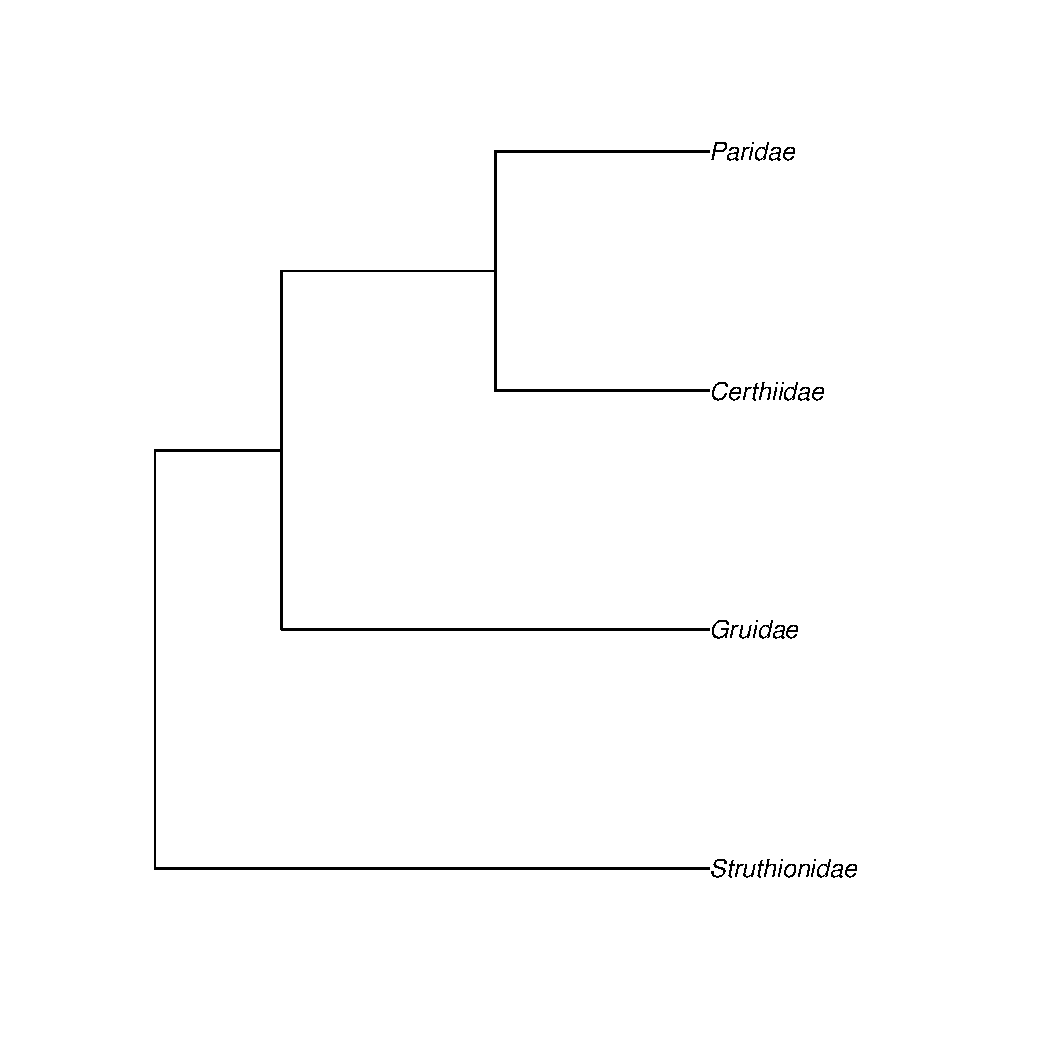
\includegraphics[width=\maxwidth]{figure/unnamed-chunk-19-1} 

\end{knitrout}

OK, it makes some sense, but also does not look perfect. Let's see how well the distribution of random levels fits a normal distribution using a qqplot:
\begin{knitrout}
\definecolor{shadecolor}{rgb}{0.969, 0.969, 0.969}\color{fgcolor}\begin{kframe}
\begin{alltt}
\hlkwd{qqnorm}\hlstd{(}\hlkwd{unlist}\hlstd{(}\hlkwd{ranef}\hlstd{(mm0)))}
\hlkwd{qqline}\hlstd{(}\hlkwd{unlist}\hlstd{(}\hlkwd{ranef}\hlstd{(mm0)),} \hlkwc{col} \hlstd{=} \hlnum{2}\hlstd{)}
\end{alltt}
\end{kframe}
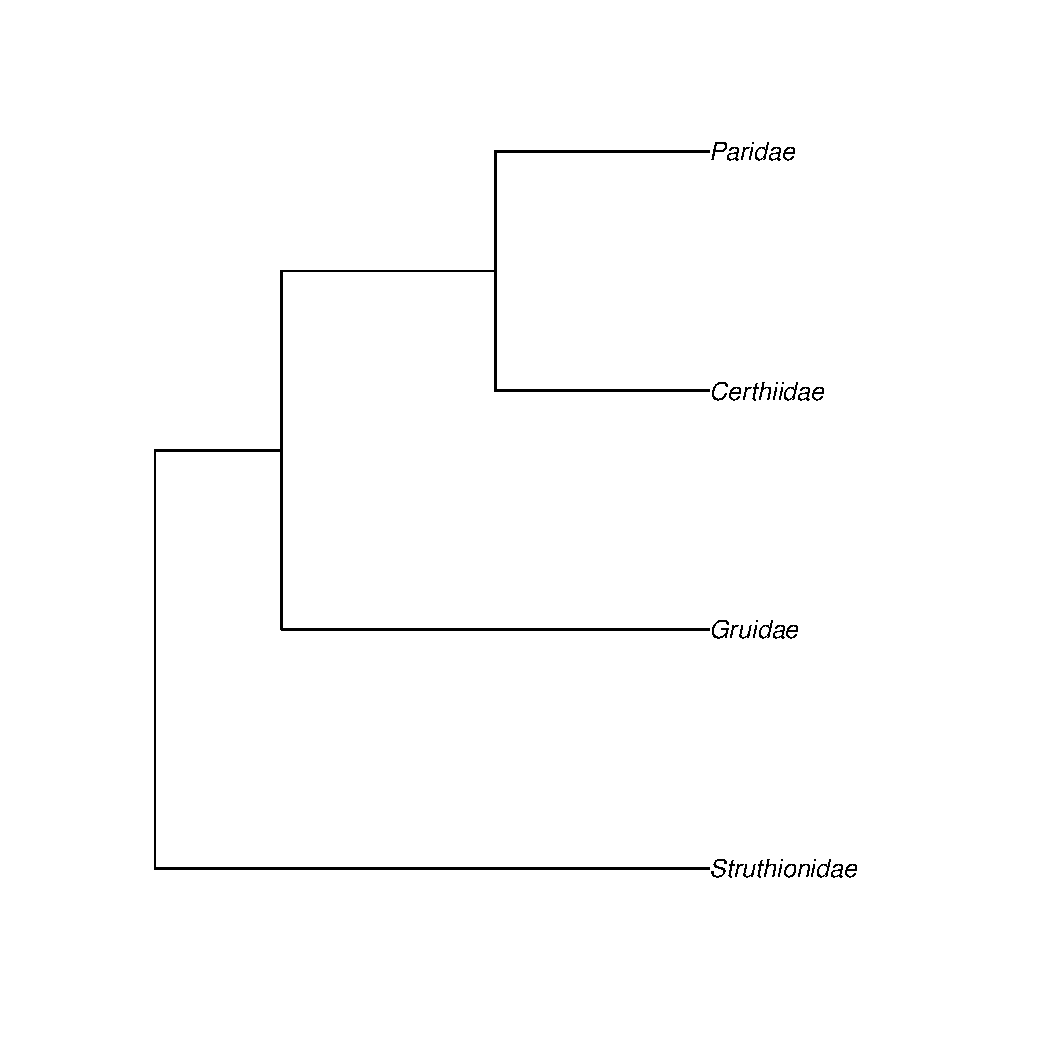
\includegraphics[width=\maxwidth]{figure/unnamed-chunk-20-1} 

\end{knitrout}
Not too bad, but with only 50 samples it is not surprising we do not get a perfect fit.

Now, let's visualize the "median" regression line, that is, the line predicted when the random deviaiton is zero, or in other words using only fixed effects and ignoring the random effect. Let's also colour points by site:
\begin{knitrout}
\definecolor{shadecolor}{rgb}{0.969, 0.969, 0.969}\color{fgcolor}\begin{kframe}
\begin{alltt}
\hlkwd{plot}\hlstd{(biggerdata}\hlopt{$}\hlstd{predictor, biggerdata}\hlopt{$}\hlstd{response,} \hlkwc{col}\hlstd{=}\hlkwd{rainbow}\hlstd{(}\hlnum{50}\hlstd{)[biggerdata}\hlopt{$}\hlstd{site])}
\hlkwd{abline}\hlstd{(}\hlkwd{fixef}\hlstd{(mm0)[}\hlnum{1}\hlstd{],} \hlkwd{fixef}\hlstd{(mm0)[}\hlnum{2}\hlstd{],} \hlkwc{lwd}\hlstd{=}\hlnum{5}\hlstd{)}
\end{alltt}
\end{kframe}
\includegraphics[width=\maxwidth]{figure/unnamed-chunk-21-1} 

\end{knitrout}

Now, let's add one thin regression line for each site, using the output of \texttt{ranef()} to get a sort of estimate of the site deviation:
\begin{knitrout}
\definecolor{shadecolor}{rgb}{0.969, 0.969, 0.969}\color{fgcolor}\begin{kframe}
\begin{alltt}
\hlkwd{plot}\hlstd{(biggerdata}\hlopt{$}\hlstd{predictor, biggerdata}\hlopt{$}\hlstd{response,} \hlkwc{col}\hlstd{=}\hlkwd{rainbow}\hlstd{(}\hlnum{50}\hlstd{)[biggerdata}\hlopt{$}\hlstd{site])}
\hlkwd{abline}\hlstd{(}\hlkwd{fixef}\hlstd{(mm0)[}\hlnum{1}\hlstd{],} \hlkwd{fixef}\hlstd{(mm0)[}\hlnum{2}\hlstd{],} \hlkwc{lwd}\hlstd{=}\hlnum{5}\hlstd{)}

\hlkwa{for} \hlstd{(i} \hlkwa{in} \hlnum{1}\hlopt{:}\hlnum{50}\hlstd{)}
\hlstd{\{}
  \hlkwd{abline}\hlstd{(}\hlkwc{a} \hlstd{=} \hlkwd{fixef}\hlstd{(mm0)[}\hlnum{1}\hlstd{]}\hlopt{+}\hlkwd{unlist}\hlstd{(}\hlkwd{ranef}\hlstd{(mm0))[i],}
         \hlkwc{b} \hlstd{=} \hlkwd{fixef}\hlstd{(mm0)[}\hlnum{2}\hlstd{],} \hlkwc{lwd}\hlstd{=}\hlnum{1}\hlstd{,} \hlkwc{col}\hlstd{=}\hlkwd{rainbow}\hlstd{(}\hlnum{50}\hlstd{)[i])}
\hlstd{\}}

\hlstd{x} \hlkwb{<-} \hlkwd{seq}\hlstd{(}\hlopt{-}\hlnum{4}\hlopt{*}\hlkwd{sqrt}\hlstd{(rvar),}\hlnum{4}\hlopt{*}\hlkwd{sqrt}\hlstd{(rvar),}\hlkwd{sqrt}\hlstd{(rvar)}\hlopt{/}\hlnum{100}\hlstd{)}

\hlstd{dens} \hlkwb{<-} \hlkwd{as.matrix}\hlstd{(}\hlkwd{cbind}\hlstd{(x,}\hlnum{10}\hlopt{*}\hlkwd{dnorm}\hlstd{(}\hlkwc{x} \hlstd{= x,} \hlkwc{mean} \hlstd{=}\hlnum{0} \hlstd{,} \hlkwc{sd} \hlstd{=} \hlkwd{sqrt}\hlstd{(rvar))))}
\hlstd{dens[,}\hlnum{1}\hlstd{]} \hlkwb{<-} \hlstd{dens[,}\hlnum{1}\hlstd{]} \hlopt{-} \hlkwd{mean}\hlstd{(dens[,}\hlnum{1}\hlstd{])}
\hlstd{dens[,}\hlnum{2}\hlstd{]} \hlkwb{<-} \hlstd{dens[,}\hlnum{2}\hlstd{]} \hlopt{-} \hlkwd{mean}\hlstd{(dens[,}\hlnum{2}\hlstd{])}

\hlcom{# library(spdep)}
\hlcom{# plot(Rotation(dens, -0.99*pi/2))}
\hlcom{# }
\hlcom{# plot(dens)}
\hlcom{# theta <- -pi/2}
\hlcom{# k <- 1}
\hlcom{# newcoor <- k * dens %*% matrix(c(cos(theta),-sin(theta),sin(theta),cos(theta)), 2, 2)}
\hlcom{# plot(0.5*newcoor[,1], 10*newcoor[,2]+fixef(mm0)[1], lwd=3)}
\hlcom{# }
\hlstd{theta} \hlkwb{<-} \hlopt{-}\hlnum{0.95}\hlopt{*}\hlstd{pi}\hlopt{/}\hlnum{2}
\hlstd{k} \hlkwb{<-} \hlnum{1}
\hlstd{newcoor} \hlkwb{<-} \hlstd{k} \hlopt{*} \hlstd{dens} \hlopt \hlkwd{matrix}\hlstd{(}\hlkwd{c}\hlstd{(}\hlkwd{cos}\hlstd{(theta),}\hlopt{-}\hlkwd{sin}\hlstd{(theta),}\hlkwd{sin}\hlstd{(theta),}\hlkwd{cos}\hlstd{(theta)),} \hlnum{2}\hlstd{,} \hlnum{2}\hlstd{)}
\hlkwd{lines}\hlstd{(newcoor[,}\hlnum{1}\hlstd{]}\hlopt{+}\hlnum{2}\hlstd{,} \hlnum{1}\hlopt{+}\hlstd{newcoor[,}\hlnum{2}\hlstd{]}\hlopt{+}\hlkwd{fixef}\hlstd{(mm0)[}\hlnum{1}\hlstd{],} \hlkwc{lwd}\hlstd{=}\hlnum{3}\hlstd{)}
\end{alltt}
\end{kframe}
\includegraphics[width=\maxwidth]{figure/unnamed-chunk-22-1} 

\end{knitrout}


\begin{tcolorbox}[colback=green!5,colframe=green!40!black,title=Fixed or random effect?]
When you want to include a categorical variable as a predictor in a model you can generally 
\begin{itemize}
\item First, if the predictor is a numerical variable (like size, temperature, number of species\dots) you will generally want a fixed effect, because the order and distance between values is likely meaningful. A random effect consider values as random "names" for grouping levels.
\item In general it does not change inference much. Random effects are slightly more efficient because the differences between grouping levels are assumed to come from a normal distribution, instead of being estimated independently from each other. 
\item A slightly lame but practical reason to use random effects: models output are cleaner with random effects because you get a single parameter estimate for a grouping variable modeled as a random effect, instead of a parameter estimate for each level of the grouping variable when modeled with a fixed effect.
\item Using a random effect instead of a fixed effect shifts the focus from the effect of each grouping level to variation among grouping levels. What is more interesting to you?
\item Often we use random effect to "correct" for some structure in the data that is not of interest. But random variance parameters can be of interest in themselves. For instance they can quantify genetic variation, individual repeatability, niche specialisation\dots if a variance parameter is of interest then estimate it using a random effect.
\item On the other hand, if you are very interested in how different a particular grouping level is from other levels, use fixed effects.
\item Be careful with random effects if the number of grouping levels is small. You definitely need at least 3, probably at least 5, maybe at least 10\dots With few grouping levels the fitting algorithm could have difficulties estimating the random variance, leading to unstable results (you may get different results from different algorithms) or the random variance being estimated to exactly zero.
\end{itemize}
\end{tcolorbox}



\section{Confidence intervals and Tests}
Sometimes random effects are part of the experimental design and are in the models only to control for confounding effects. But sometimes we care about the value of variance components or we want to report their statistical significance. Let's try a few approaches to evaluate the significance of a random effect. 


\begin{Exercise}[difficulty=1, title={CI for variance components in lme4}]
Use the function \texttt{confint} to estimate confidence intervals for the variance component for "site". Hints: 1) by default confint calculate 95\% confidence intervals for all fixed and random effects as well as for the residual standard deviation which is labelled ".sigma"; 2) confint returns standard deviations for random effects, instead of variances. Take the square of a standard deviation to obtain a variance.
\end{Exercise}
\begin{Answer}
\begin{knitrout}
\definecolor{shadecolor}{rgb}{0.969, 0.969, 0.969}\color{fgcolor}\begin{kframe}
\begin{alltt}
\hlstd{lmm1} \hlkwb{<-} \hlkwd{lmer}\hlstd{(herbivory} \hlopt{~} \hlstd{thorndensity} \hlopt{+} \hlstd{(}\hlnum{1}\hlopt{|}\hlstd{site),} \hlkwc{data}\hlstd{=thorns)}
\hlstd{conf} \hlkwb{<-} \hlkwd{confint}\hlstd{(lmm1)}
\end{alltt}


{\ttfamily\noindent\itshape\color{messagecolor}{\#\# Computing profile confidence intervals ...}}\begin{alltt}
\hlstd{conf[}\hlnum{1}\hlstd{,]}\hlopt{^}\hlnum{2}
\end{alltt}
\begin{verbatim}
##  2.5 % 97.5 % 
## 0.5247 8.1932
\end{verbatim}
\end{kframe}
\end{knitrout}
\end{Answer}


\begin{Exercise}[difficulty=1, title={Testing variance components in lme4}]
Use the function anova to test the statistical significance of the random effect "site" in the thorn dataset. Hint: 1) you need to fit a simple linear model (lm()) without site to serve as a null model against which to compare your mixed model. The function anova() need to compare two models in this case. 2) the order in which you give your models to anova() matters.
\end{Exercise}
\begin{Answer}
\begin{knitrout}
\definecolor{shadecolor}{rgb}{0.969, 0.969, 0.969}\color{fgcolor}\begin{kframe}
\begin{alltt}
\hlstd{lm0} \hlkwb{<-} \hlkwd{lm}\hlstd{(herbivory} \hlopt{~} \hlstd{thorndensity ,} \hlkwc{data}\hlstd{=thorns)}
\hlstd{lmm1} \hlkwb{<-} \hlkwd{lmer}\hlstd{(herbivory} \hlopt{~} \hlstd{thorndensity} \hlopt{+} \hlstd{(}\hlnum{1}\hlopt{|}\hlstd{site),} \hlkwc{data}\hlstd{=thorns)}

\hlkwd{anova}\hlstd{(lm0, lmm1)}\hlcom{#doesn't work!}
\end{alltt}


{\ttfamily\noindent\bfseries\color{errorcolor}{\#\# Error: \$ operator not defined for this S4 class}}\begin{alltt}
\hlkwd{anova}\hlstd{(lmm1, lm0)}\hlcom{# mixed model must go first!}
\end{alltt}


{\ttfamily\noindent\itshape\color{messagecolor}{\#\# refitting model(s) with ML (instead of REML)}}\begin{verbatim}
## Data: thorns
## Models:
## lm0: herbivory ~ thorndensity
## lmm1: herbivory ~ thorndensity + (1 | site)
##      Df AIC BIC logLik deviance Chisq Chi Df Pr(>Chisq)    
## lm0   3 224 231   -109      218                            
## lmm1  4 172 182    -82      164  53.4      1    2.7e-13 ***
## ---
## Signif. codes:  0 '***' 0.001 '**' 0.01 '*' 0.05 '.' 0.1 ' ' 1
\end{verbatim}
\end{kframe}
\end{knitrout}
The p-value you get is \ensuremath{2.6595\times 10^{-13}}, however, be aware this is a conservative estimate!

A better option could be to use the RLRsim which performs simulation-based tests which should be more correct when variances are close to zero:
\begin{knitrout}
\definecolor{shadecolor}{rgb}{0.969, 0.969, 0.969}\color{fgcolor}\begin{kframe}
\begin{alltt}
\hlkwd{library}\hlstd{(RLRsim)}
\hlcom{## compare m0 and m1}
\hlkwd{exactLRT}\hlstd{(lmm1, lm0)}
\end{alltt}


{\ttfamily\noindent\itshape\color{messagecolor}{\#\# No restrictions on fixed effects. REML-based inference preferable.}}

{\ttfamily\noindent\itshape\color{messagecolor}{\#\# Using likelihood evaluated at REML estimators.}}

{\ttfamily\noindent\itshape\color{messagecolor}{\#\# Please refit model with method="{}ML"{} for exact results.}}\begin{verbatim}
## 
## 	simulated finite sample distribution of LRT. (p-value based on 10000
## 	simulated values)
## 
## data:  
## LRT = 53, p-value <2e-16
\end{verbatim}
\end{kframe}
\end{knitrout}

\end{Answer}
If you have managed to solve this exercise, congrats! What you have done is called a Likelihood Ratio Test (LRT). This is a useful test, but be careful, the models you compare need to be nested, that is, one model is a special case of the other one. In our case the lm() is nested within the lmer() model because in the special case when the variance in the random effect (1|site) is exactly zero the two models are identical.
Also, be aware that for random effects Likelihood Ratio Tests using anova are generally conservative.



\begin{tcolorbox}[colback=green!5,colframe=green!40!black,title=How does random effect formula work again?]
Random effect formula in lme4 and many other R-packages look like (1$|$group).

On the right-hand side of the pipe ($|$) is the variable that groups data points; for instance location, time, species\dots \\

On the left-hand side of the pipe is what varies according to grouping. In today's example we use only $1$, which stands for \textbf{intercept}. In other words we use random-intercept models. You can write other things on the left-hand side to define more complex models ("random interactions", "random regressions",\dots) but we will see that next time.

\end{tcolorbox}




\section{}


\begin{Exercise}[difficulty=1, title={xxx}]

\end{Exercise}
\begin{Answer}

\end{Answer}


\begin{Exercise}[difficulty=3, title={Do kangaroos have personalities?}]

We want to know whether the distance at which kangaroos run away when we approach is different among individuals. Load the dataset "roo.csv" and fit linear mixed models of "EscapeDistance" to find out. We can quantify how much individuals differ from each other using repeatability. Repeatability can be defined as the ratio of variance among individuals over the sum variance among individuals plus variance within individuals. 

We can estimate the variance among individuals with a random effect of \texttt{id} (individual identifier) and the variance within individuals can be estimated as the residual variance. 

What other variables to include? Does individual repeatability explain more variance than expected by randomly grouping observations? What is the repeatability of behaviour?
\end{Exercise}
\begin{Answer}
\begin{knitrout}
\definecolor{shadecolor}{rgb}{0.969, 0.969, 0.969}\color{fgcolor}\begin{kframe}
\begin{alltt}
\hlstd{roo} \hlkwb{<-} \hlkwd{read.csv}\hlstd{(}\hlstr{"Data/roo.csv"}\hlstd{)}
\end{alltt}
\end{kframe}
\end{knitrout}

There is no simple answer to what model you should fit, because it depends what you think is part of intrinsic individual differences and what is not. The simplest model would be:
\begin{knitrout}
\definecolor{shadecolor}{rgb}{0.969, 0.969, 0.969}\color{fgcolor}\begin{kframe}
\begin{alltt}
\hlkwd{summary}\hlstd{(}\hlkwd{lmer}\hlstd{(EscapeDistance} \hlopt{~} \hlnum{1} \hlopt{+} \hlstd{(}\hlnum{1}\hlopt{|}\hlstd{id)} \hlopt{+} \hlstd{(}\hlnum{1}\hlopt{|}\hlstd{Year),} \hlkwc{data}\hlstd{=roo))}
\end{alltt}
\begin{verbatim}
## Linear mixed model fit by REML ['lmerMod']
## Formula: EscapeDistance ~ 1 + (1 | id) + (1 | Year)
##    Data: roo
## 
## REML criterion at convergence: 19646
## 
## Scaled residuals: 
##    Min     1Q Median     3Q    Max 
## -5.229 -0.441  0.038  0.489  5.131 
## 
## Random effects:
##  Groups   Name        Variance Std.Dev.
##  id       (Intercept) 125.7    11.21   
##  Year     (Intercept)  64.4     8.03   
##  Residual              23.4     4.83   
## Number of obs: 2909, groups:  id, 826; Year, 8
## 
## Fixed effects:
##             Estimate Std. Error t value
## (Intercept)    33.38       2.87    11.6
\end{verbatim}
\end{kframe}
\end{knitrout}
That's not necessarily wrong, but be aware of what residual and id variance contain here: age, sex, date, location... should they?

The following model is probably too complex:
\begin{knitrout}
\definecolor{shadecolor}{rgb}{0.969, 0.969, 0.969}\color{fgcolor}\begin{kframe}
\begin{alltt}
\hlkwd{summary}\hlstd{(}\hlkwd{lmer}\hlstd{(EscapeDistance} \hlopt{~} \hlnum{1} \hlopt{+} \hlstd{Sex} \hlopt{+} \hlkwd{as.factor}\hlstd{(Age3)} \hlopt{+} \hlstd{(}\hlnum{1}\hlopt{|}\hlstd{id)} \hlopt{+} \hlstd{(}\hlnum{1}\hlopt{|}\hlstd{Mother)} \hlopt{+} \hlstd{(}\hlnum{1}\hlopt{|}\hlstd{Year),} \hlkwc{data}\hlstd{=roo))}
\end{alltt}
\begin{verbatim}
## Linear mixed model fit by REML ['lmerMod']
## Formula: EscapeDistance ~ 1 + Sex + as.factor(Age3) + (1 | id) + (1 |  
##     Mother) + (1 | Year)
##    Data: roo
## 
## REML criterion at convergence: 16967
## 
## Scaled residuals: 
##    Min     1Q Median     3Q    Max 
## -3.988 -0.540 -0.006  0.597  6.935 
## 
## Random effects:
##  Groups   Name        Variance Std.Dev.
##  id       (Intercept) 10.31    3.211   
##  Mother   (Intercept)  2.42    1.556   
##  Year     (Intercept)  0.69    0.831   
##  Residual             14.30    3.781   
## Number of obs: 2909, groups:  id, 826; Mother, 197; Year, 8
## 
## Fixed effects:
##                  Estimate Std. Error t value
## (Intercept)        24.537      0.402   61.07
## SexMale             1.781      0.300    5.93
## as.factor(Age3)1   14.799      0.233   63.41
## as.factor(Age3)2   18.645      0.389   47.88
## as.factor(Age3)3   21.342      1.207   17.68
## 
## Correlation of Fixed Effects:
##             (Intr) SexMal a.(A3)1 a.(A3)2
## SexMale     -0.383                       
## as.fct(A3)1 -0.255  0.121                
## as.fct(A3)2 -0.180  0.094  0.550         
## as.fct(A3)3 -0.074  0.036  0.218   0.232
\end{verbatim}
\end{kframe}
\end{knitrout}
indeed, "sex" and "Mother" (identity of an individual's mother) are part of an individual identity. Correcting for those will likely reduce the id variance. However, I think it makes sense to correct for age.


Maybe a good model would be:
\begin{knitrout}
\definecolor{shadecolor}{rgb}{0.969, 0.969, 0.969}\color{fgcolor}\begin{kframe}
\begin{alltt}
\hlkwd{summary}\hlstd{(}\hlkwd{lmer}\hlstd{(EscapeDistance} \hlopt{~} \hlnum{1} \hlopt{+} \hlkwd{as.factor}\hlstd{(Age3)} \hlopt{+} \hlstd{Julian} \hlopt{+} \hlstd{(}\hlnum{1}\hlopt{|}\hlstd{Year)} \hlopt{+} \hlstd{(}\hlnum{1}\hlopt{|}\hlstd{id) ,} \hlkwc{data}\hlstd{=roo))}
\end{alltt}
\begin{verbatim}
## Linear mixed model fit by REML ['lmerMod']
## Formula: EscapeDistance ~ 1 + as.factor(Age3) + Julian + (1 | Year) +  
##     (1 | id)
##    Data: roo
## 
## REML criterion at convergence: 16982
## 
## Scaled residuals: 
##    Min     1Q Median     3Q    Max 
## -3.789 -0.570  0.004  0.568  6.828 
## 
## Random effects:
##  Groups   Name        Variance Std.Dev.
##  id       (Intercept) 13.236   3.638   
##  Year     (Intercept)  0.823   0.907   
##  Residual             13.985   3.740   
## Number of obs: 2909, groups:  id, 826; Year, 8
## 
## Fixed effects:
##                  Estimate Std. Error t value
## (Intercept)      19.28062    0.78097   24.69
## as.factor(Age3)1 16.20258    0.24313   66.64
## as.factor(Age3)2 20.43964    0.39803   51.35
## as.factor(Age3)3 23.78528    1.20335   19.77
## Julian            0.02646    0.00285    9.29
## 
## Correlation of Fixed Effects:
##             (Intr) a.(A3)1 a.(A3)2 a.(A3)3
## as.fct(A3)1 -0.503                        
## as.fct(A3)2 -0.382  0.581                 
## as.fct(A3)3 -0.169  0.244   0.253         
## Julian      -0.877  0.443   0.346   0.154
\end{verbatim}
\end{kframe}
\end{knitrout}
(but it is not unambiguous; you can disagree).

From there, we can test the statistical significance of repeatability as:
\begin{knitrout}
\definecolor{shadecolor}{rgb}{0.969, 0.969, 0.969}\color{fgcolor}\begin{kframe}
\begin{alltt}
\hlstd{lmfull} \hlkwb{<-} \hlkwd{lmer}\hlstd{(EscapeDistance} \hlopt{~} \hlnum{1} \hlopt{+} \hlkwd{as.factor}\hlstd{(Age3)} \hlopt{+} \hlstd{Julian} \hlopt{+} \hlstd{(}\hlnum{1}\hlopt{|}\hlstd{Year)} \hlopt{+} \hlstd{(}\hlnum{1}\hlopt{|}\hlstd{id) ,} \hlkwc{data}\hlstd{=roo)}
\hlstd{lmreduced} \hlkwb{<-} \hlkwd{lmer}\hlstd{(EscapeDistance} \hlopt{~} \hlnum{1} \hlopt{+} \hlkwd{as.factor}\hlstd{(Age3)} \hlopt{+} \hlstd{Julian} \hlopt{+} \hlstd{(}\hlnum{1}\hlopt{|}\hlstd{Year) ,} \hlkwc{data}\hlstd{=roo)}
\hlkwd{anova}\hlstd{(lmfull, lmreduced)}
\end{alltt}


{\ttfamily\noindent\itshape\color{messagecolor}{\#\# refitting model(s) with ML (instead of REML)}}\begin{verbatim}
## Data: roo
## Models:
## lmreduced: EscapeDistance ~ 1 + as.factor(Age3) + Julian + (1 | Year)
## lmfull: EscapeDistance ~ 1 + as.factor(Age3) + Julian + (1 | Year) + 
## lmfull:     (1 | id)
##           Df   AIC   BIC logLik deviance Chisq Chi Df Pr(>Chisq)    
## lmreduced  7 17793 17834  -8889    17779                            
## lmfull     8 16988 17036  -8486    16972   806      1     <2e-16 ***
## ---
## Signif. codes:  0 '***' 0.001 '**' 0.01 '*' 0.05 '.' 0.1 ' ' 1
\end{verbatim}
\end{kframe}
\end{knitrout}

and estimate repeatability:
\begin{knitrout}
\definecolor{shadecolor}{rgb}{0.969, 0.969, 0.969}\color{fgcolor}\begin{kframe}
\begin{alltt}
\hlkwd{as.numeric}\hlstd{(}\hlkwd{VarCorr}\hlstd{(lmfull)[}\hlnum{1}\hlstd{])}\hlopt{/}\hlstd{(}\hlkwd{as.numeric}\hlstd{(}\hlkwd{VarCorr}\hlstd{(lmfull)[}\hlnum{1}\hlstd{])}\hlopt{+}
                                  \hlkwd{as.numeric}\hlstd{(}\hlkwd{VarCorr}\hlstd{(lmfull)[}\hlnum{2}\hlstd{])}\hlopt{+}
                                  \hlkwd{sigma}\hlstd{(lmfull)}\hlopt{^}\hlnum{2}\hlstd{)}
\end{alltt}
\begin{verbatim}
## [1] 0.472
\end{verbatim}
\end{kframe}
\end{knitrout}

\end{Answer}

\section{More resources}


\href{http://bbolker.github.io/mixedmodels-misc/glmmFAQ.html}{Ben Bolker's GLMM FAQ is a gold mine if you need some technical details about mixed models (generalized or not).}

If you are going to do lots of mixed models consider subscribing to the mailing-list \href{https://stat.ethz.ch/mailman/listinfo/r-sig-mixed-models}{https://stat.ethz.ch/mailman/listinfo/r-sig-mixed-models}, ask questions or search the archive (anyway, Google is likely to directly send you to the archive).



\end{document}
